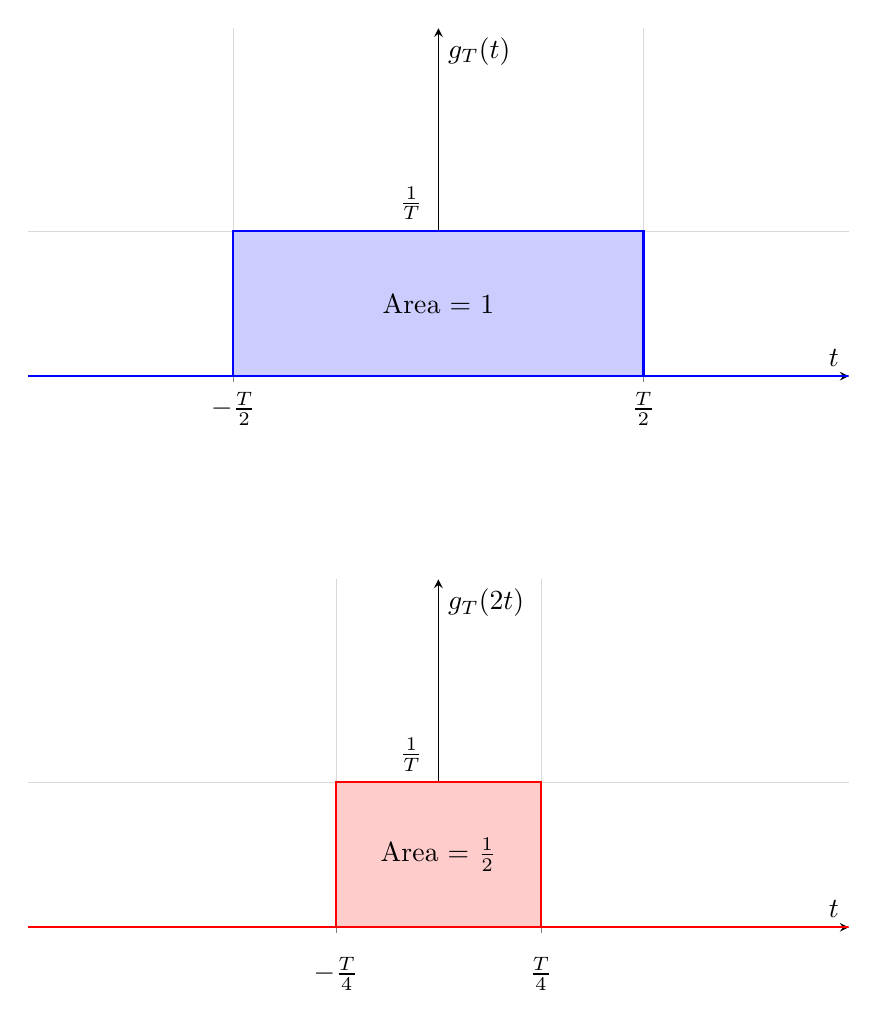
\begin{tikzpicture}
	%#################################################
	%### Top Plot: The original pulse g_T(t)
	%#################################################
	\begin{scope}[yshift=7cm]
		\begin{axis}[
			width=12cm,
			yticklabel style={yshift=10pt},
			height=6cm,
			axis lines=middle,
			xlabel={$t$},
			ylabel={$g_T(t)$},
			ymin=0, ymax=1.2,
			xmin=-2, xmax=2,
			grid=major,
			grid style={line width=.1pt, draw=gray!30},
			% removed: no marks (invalid axis key)
			xtick={-1, 1},
			xticklabels={$-\frac{T}{2}$, $\frac{T}{2}$},
			ytick={0.5},
			yticklabels={$\frac{1}{T}$},
			]
			% Plot the pulse and fill it with color
			\addplot[blue, thick, fill=blue!20, mark=none] coordinates {
				(-2,0) (-1,0) (-1,0.5) (1,0.5) (1,0) (2,0)
			} \closedcycle;
			% Add the area annotation
			\node at (axis cs:0, 0.25) {Area = $1$};
		\end{axis}
	\end{scope}
	
	%#################################################
	%### Bottom Plot: The time-scaled pulse g_T(2t)
	%#################################################
	\begin{scope}[yshift=0cm]
		\begin{axis}[
						yticklabel style={yshift=10pt},
			width=12cm,
			height=6cm,
			axis lines=middle,
			xlabel={$t$},
			ylabel={$g_T(2t)$},
			ymin=0, ymax=1.2,
			xmin=-2, xmax=2,
			grid=major,
			grid style={line width=.1pt, draw=gray!30},
			% removed: no marks (invalid axis key)
			xtick={-0.5, 0.5},
			xticklabels={$-\frac{T}{4}$, $\frac{T}{4}$},
			ytick={0.5},
			yticklabels={$\frac{1}{T}$},
			xticklabel style={yshift=-5pt},
			]
			% Plot the compressed pulse
			\addplot[red, thick, fill=red!20, mark=none] coordinates {
				(-2,0) (-0.5,0) (-0.5,0.5) (0.5,0.5) (0.5,0) (2,0)
			} \closedcycle;
			% Add the new area annotation
			\node at (axis cs:0, 0.25) {Area = $\frac{1}{2}$};
		\end{axis}
	\end{scope}
\end{tikzpicture}
